%!TEX root = ../main.tex
\subsection{Accessing CAN Controller from Linux}\label{sec:methods_to_implement_can}
\mikkel{Changed by Catalin and a little of Mikkel :D}
Utilizing the XCanPs from bare-metal code is not enough for all nodes as some needs to run Linux as described in the analysis part.
This section describes the steps tried in order gain access to the CAN controller from Linux. 
According to Xilinx documentation, this can be done by following their Linux CAN driver guide \cite{Xilinx_wiki_Linux_CAN_driver}.
%The steps for this were to modify certain files related to the kernel configurations and the device tree settings.

\subsubsection*{Enabling the CAN Controller Drivers}
\thomas{spelling mistake -withe}
To access the CAN controller the appropriate drivers needs to be enabled in the Kernel.
Specifically, the Kconfig file withe the path shown in code \ref{code:can_kconfig_pathfile} needed to be configured.
The entry at line 128 was changed as seen in code \ref{code:can_kconfig_contents_line128}.
Originally, lines 130 and 131 were as seen in code \ref{code:can_kconfig_original_line130}.

\begin{lstlisting}[caption={CAN Kconfig pathfile.},numbers=none,label=code:can_kconfig_pathfile]
/usr/src/kernels/3.12.0-xillinux-1.3/drivers/net/can
\end{lstlisting}

\begin{lstlisting}[firstnumber=128,caption={Kconfig file contents from line 128.},label={code:can_kconfig_contents_line128}]
config CAN_XILINXCAN
	tristate "Xilinx(*@ @*)CAN"
	depends on NET [=y] && CAN_DEV [=y] && CAN [=y] && 
        (ARCH_ZYNQ || MICROBLAZE [=y])
	default y
\end{lstlisting}

\begin{lstlisting}[firstnumber=130,caption={Original content of lines 130 and 131.},label={code:can_kconfig_original_line130}]
	depends on CAN && (ARCH_ZYNQ || MICROBLAZE)
	default n
\end{lstlisting}

Unfortunately, the above steps did not enable the drivers successfully.

\subsubsection*{Changing Device Tree Settings}
The next step of the process was to modify the device tree settings file, requiring an entry for the CAN PS to be inserted.
The necessary file was located under the boot folder named as seen in code \ref{code:dts_file_zybo}.
The modifications can be seen in code \ref{code:dts_changes_zybo} for CAN controllers as well as for the AXI CAN core.

\begin{lstlisting}[numbers=none,caption={Device tree settings file and its path.},label={code:dts_file_zybo}]
/boot/xillinux-1.3-zybo.dts
\end{lstlisting}
\begin{lstlisting}[caption={Device tree settings changes.},label={code:dts_changes_zybo}]
zynq_can_0: can@e0008000 {
        compatible = "xlnx,zynq-can-1.0";
        clocks = <&clkc 19>, <&clkc 36>;
        clock-names = "can_clk", "pclk";
        reg = <0xe0008000 0x1000>;
        interrupts = <0 28 4>;
        interrupt-parent = <&intc>;
        tx-fifo-depth = <0x40>;
        rx-fifo-depth = <0x40>;
    };
axi_can_0: axi-can@40000000 {
        compatible = "xlnx,axi-can-1.00.a";
        clocks = <&clkc 0>, <&clkc 1>;
        clock-names = "can_clk", "s_axi_aclk";
        reg = <0x40000000 0x10000>;
        interrupt-parent = <&intc>;
        interrupts = <0 59 1>;
        tx-fifo-depth = <0x40>;
        rx-fifo-depth = <0x40>;
        };
\end{lstlisting}
It was expected that the changes took effect after rebooting the system, which was not the case.

\subsubsection*{Conclusion}
\thomas{I think unsuccesful}
After the changes, the CAN devices were still not visible in Linux and thus, accessing the CAN controllers was successful.

Research was done by the authors in why this could not be accomplished.
It was found that there were some naming inconsistencies between the guide and the Device Tree Settings file present in Linux running on the Zybo. Specifically, all the devices' names in the file are prepended with ps7.
A new set of changes with this naming convention was done, but with no success.\\

Another approach to this, was to build a newer version of the kernel containing these changes and to build an entirely new Linux system for the Zybo.
This approach was considered to be unfeasible as the kernel needed to be patched with Xillinux patches which are not compatible with a newer version of the kernel.
%The architecture can be seen in figure \ref{fig:CAN_Arch_with_AXI_CAN}.

%\begin{figure}[h!]
%	\centering
%	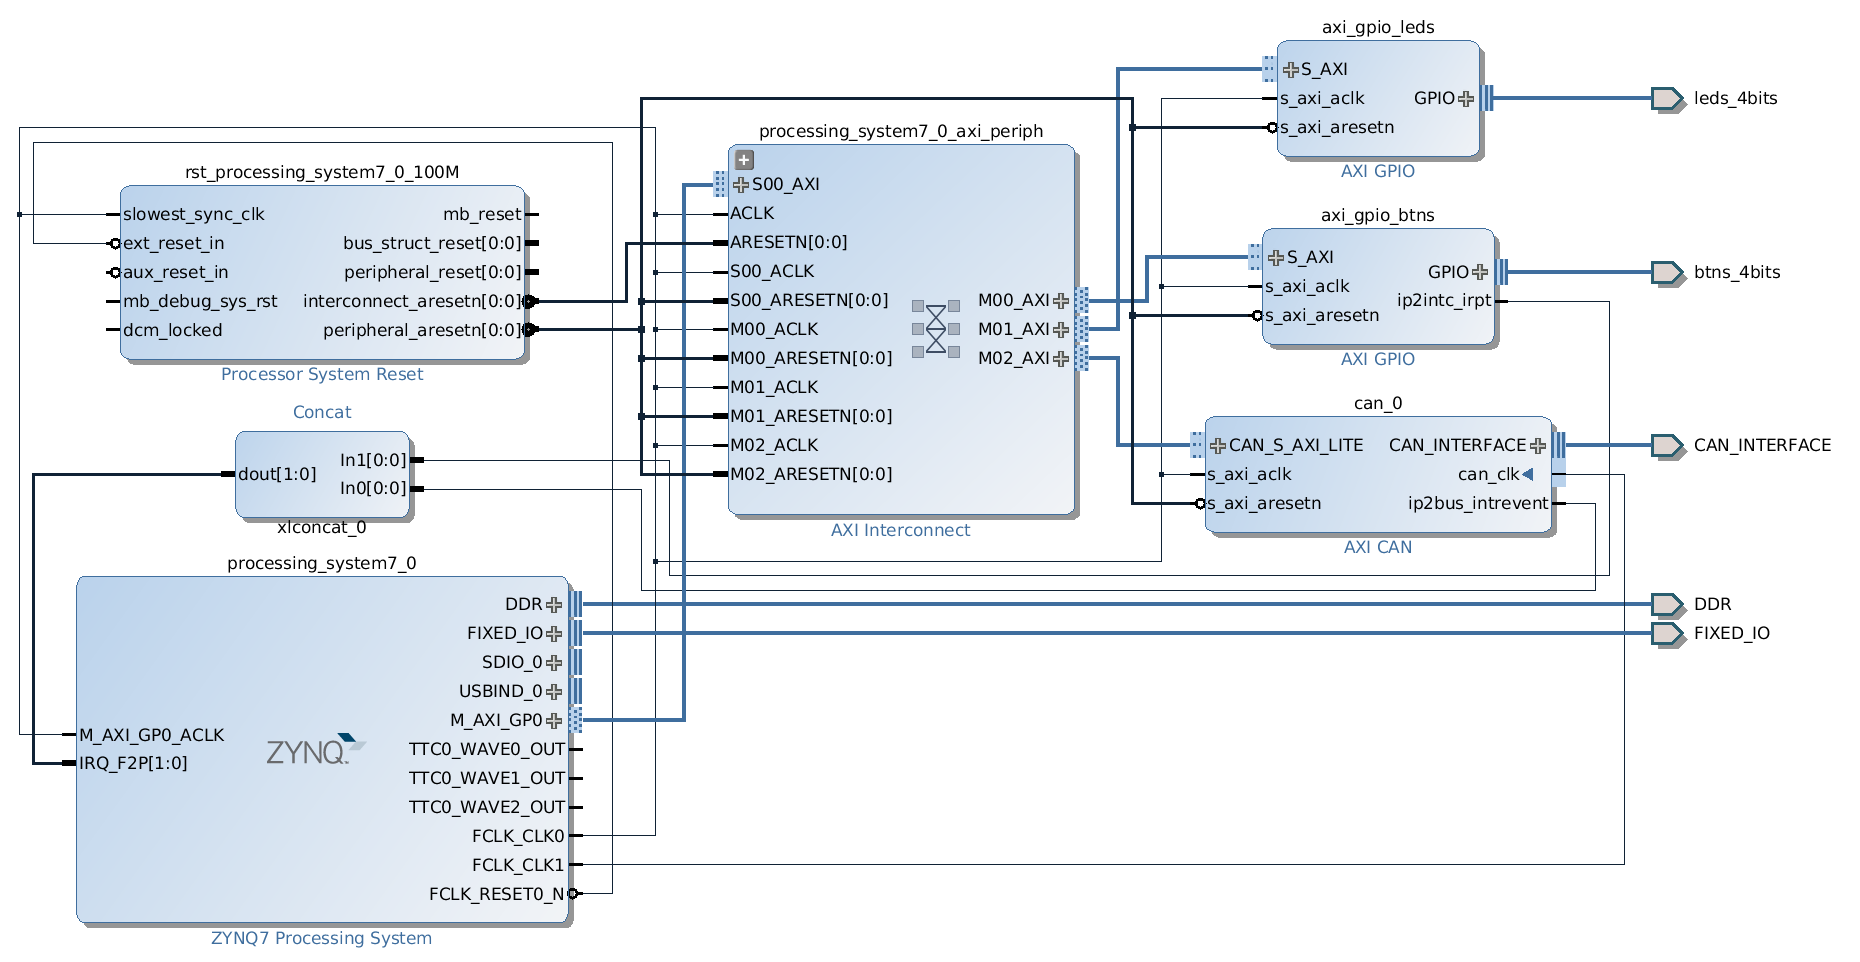
\includegraphics[width = 1.2\linewidth]{graphics/Zybo_Arch_with_AXI_CAN.png}
%	\caption{Block diagram featuring the architecture in Vivado with the AXI CAN core.}
%	\label{fig:CAN_Arch_with_AXI_CAN}
%\end{figure}
